\section{Introduction}\label{sec:introduction}

\subsection{The nature of data and information}\label{sec:information}

Terms like data or information have a very broad meaning and potentially slightly different and confusing means is different communities. \emph{Disclaimer:} The following is not an attempt to provide some sort of omnipotent information theory and only serves the applications and techniques described in this paper.

We start with the smallest pieces: \emph{atomic pieces of data} (APD). APDs do not contain other data but themselves. An APD has an \emph{identity}, \emph{value}, and \emph{data type}. The set of values of all APDs of a certain type form the \emph{defining set} of that data type. Many data types are defined through (subsets) of real or natural numbers, such as temperature values between -30 and 100 degree Celsius. A set of labels is also a typical APD type. But data types are not limited to numbers and strings. Tuples of numbers, bitmaps, graphs, etc can also be the values of APDs, but only if these APDs are never considered to consist of multiple parts. Each APD has an identity. Two APDs from type integer, are not necessarily the same just because their values are the same number.

\begin{figure}
  \centering
  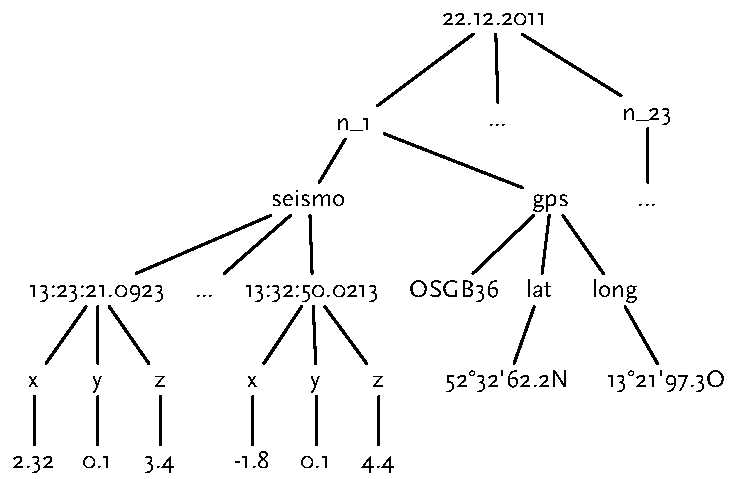
\includegraphics[width=0.65\linewidth]{figures/example_information_graph}
  \caption{Experiment data (information) from a WSN with seismo and gps sensors}
  \label{fig:example_information_graph}
\end{figure}

Because each single APD does not have any context it is considered \emph{data} and not information. But APDs can be linked to each other. We consider graphs of APDs as \emph{information}. The vertices are sets of APDs and edges connect different APDs of such a graph. In such a graph each APD has a \emph{context}: that are the neighbors of a APD.

The information graph if Fig.~\ref{fig:example_information_graph} for example comprises of all the data from an experiment with a WSN of 23 nodes and two sensors (seismo and gps). The includes APD have several types: date, time, node identifiers, sensor identifiers, spatial axis, accelerometer readings, degrees (long/lat), and coordinate reference systems. 

The APDs in a information graph are \emph{connected} if there is a path between them. In the last example, each accelerometer reading is connected to a axis, to a time, to a node, and to a date. To APDs can share connections, i.e. can be connected to the same APDs. We call the set of shared APDs for each pair of APD the \emph{common ancestors} of this pair. Two APDs are \emph{siblings} regarding to another APD if they are both connected to this APD. The intuition of these definitions are based on information shaped as a tree, but it also meant for actual graphs. 

Information has also a type (\emph{information type}). Consider the WSN from the last example: all possible information graphs from experiments with this WSN share a unique structure. There are constraints for the set of possible APDs and possible edges.

There are several technical systems to create, store, and access information. XML files can contain information trees (and graphs) where each entity (or attribute) represents an APD. XML schema define types of information. Relational databases organize information in tables and references between entries of different tables. Each value (specific entry, specific column) in a relational database table is a APD. Entries and relationships form links between APDs. Entity relationship diagrams or database schemas define types of information. Models (as in OMG) are information, objects (and attributes) are APDs. Meta-models define types of information. Within programming languages data structures (classes, structs, union, arrays and primitive types) are used to represent information. Further systems are based on ontologies or RDF.

There are several abstractions for the representation of information. We may call graphs of APDs information, but these graphs are actually only one possible abstraction. Other (some limited) representations are list, maps, functions, terms, different forms of trees and graphs, algebras, vectors, matrices, tables, etc. Of cause representations can be combined. 

\subsection{Analysis and Traces}
 
\begin{figure}
  \centering
  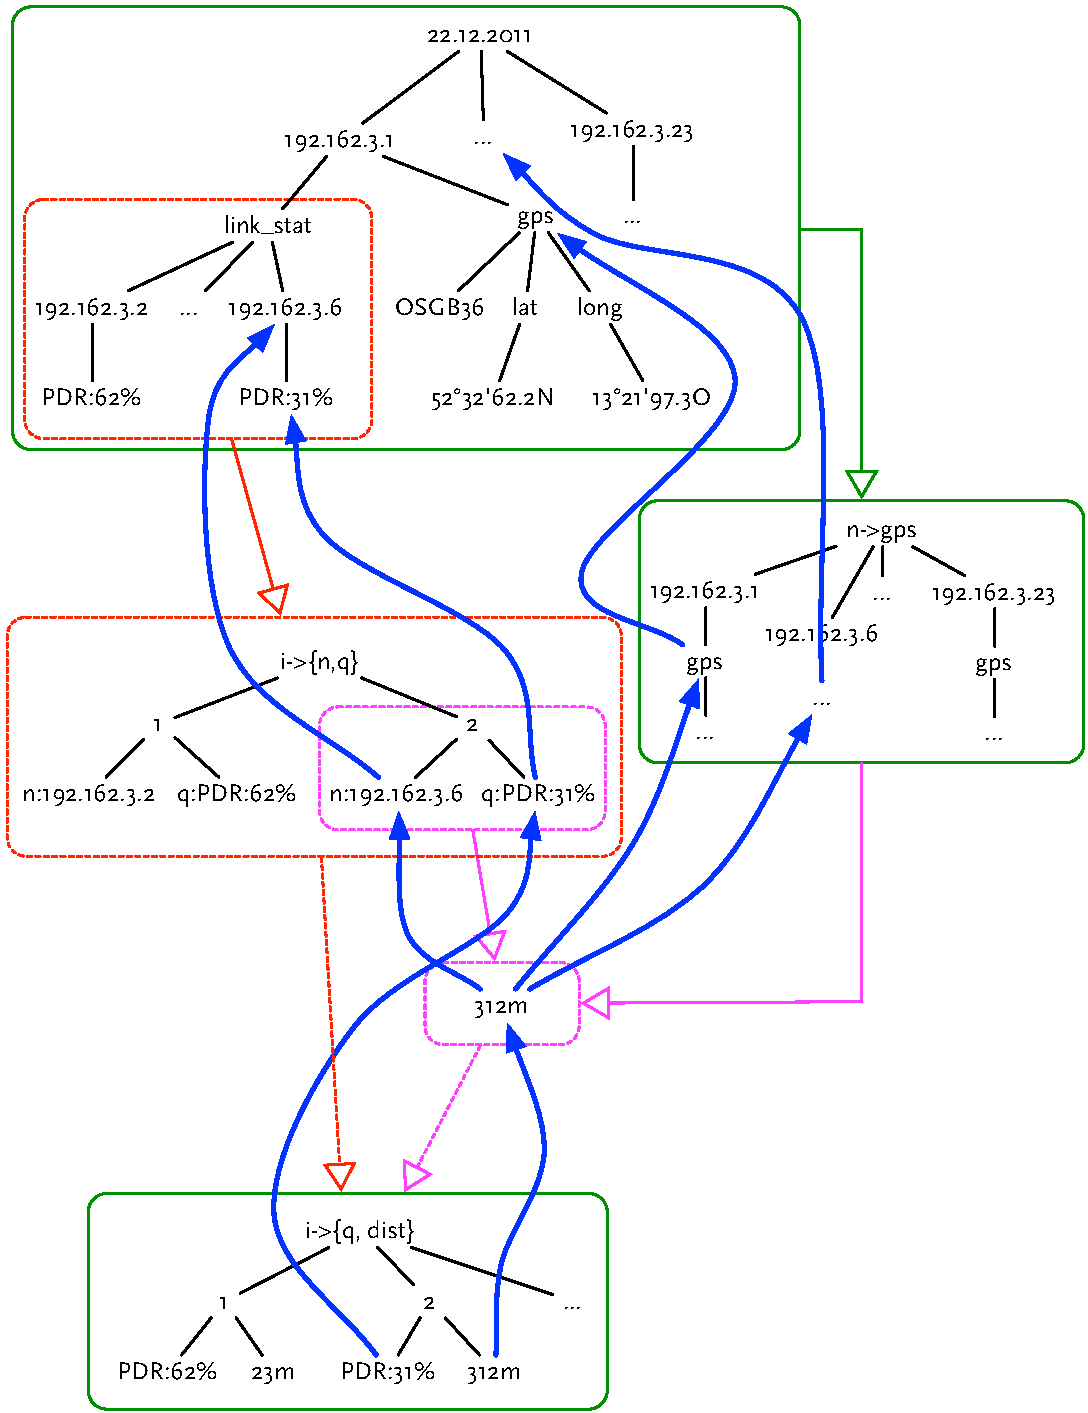
\includegraphics[width=\linewidth]{figures/example_analysis_data}
  \caption{An example for Information in different analysis steps and traces between its APDs. The example is taken from an experiment with a mesh network of wireless (802.11) nodes. The information obtained within the network includes information about links and link quality (packed delivery rate, PDR) and the position of the nodes (via global positioning system, GPS). The colored boxes mark distinct information graphs. The thin colored arrows mark analysis steps, the arrow point marks the created information graph. Green boxes mark information graphs that cover the whole data range, other colors mark information graphs that only cover a single information sample. In the example, the red box describe the links of one network node, the purple boxes describe a single link. The thick blue arrows mark traces between APDs: the arrows show which APD is based on what other APDs.}
  \label{fig:example_analysis_data}
\end{figure}

The information graphs considered in this paper (e.g. the information graphs defined and exemplified in section~\ref{sec:information}) are to be analyzed. The information covered is on a low level of abstraction and we want to extract information on a higher layer of abstraction. The term \emph{analysis} describes the process in which we create new information graphs from existing information graph. An analysis can be decided into analysis steps. In each \emph{analysis step} a distinct information graph is created. An analysis can have multiple steps and hence produce intermediate information graphs. Fig.~\ref{fig:example_analysis_data} shows the information graphs of an example analysis.

When a new information graph is created during an analysis step, APDs of the new graph can be assigned to APDs of existing information graphs. New APDs are either directly taken (copy) or are computed from one or more existing APDs. This creates a directed relationship between APDs (of different information graphs). This relationship is reflexive and antisymmetric. The transitive hull links one APD to all those APD that participate in its creation. This relation induces a partial order on the set of all APDs. We denote this relation and the partial order as \emph{trance relation} or \emph{trace order} of the respective analysis. The ordered set of APDs that participate in the creation of an APD (including the APD itself) is called the \emph{trace} of that APD. All APDs in the trace of an APD are called the \emph{ancestors} of that APD.

The edges in an information graph also provide relationships between APDs. We can create the union of all the edge relationships of all information graphs of an analysis and the trace relationship of that analysis. This relation is called \emph{extended trace} relationship. Note that this relationship does not induce an order. Two APDs are called \emph{related with respect to the traces or extended traces}, if they are both related to at least one APD via the transitive hull of the trace or extended trace relationship. The APDs that two related APDs are both related to are called the \emph{common ancestors} of those APDs. 

Extended traces can be further extended to form weak traces. Depending on the type and semantic of APDs, we can define (usually equivalence) relationships on the values of APDs. For example: to denote close proximity GPS coordinates can be designated equivalent, timestamps can be designated equivalent if they shell denote the same point in time, etc. This way, two APDs can be siblings if they share ancestors with different identity but (similar or) same meaning.

If the information graphs are trees or contain a designated tree, we call the reflexive and antisymmetric relation derived from the edges of this graph the \emph{information tree} of this information graph. We always assume that all information graphs are disjoint (all sets of vertices and edges are disjoint). When all graphs of an analysis have an information tree the union of those trees and the trace relationship is also a antisymmetric, reflexive relationship with a transitive hull. The extended trace relationship induces a partial order. There also is a partial order among all the ancestors of two (or more) APDs. Considering the ancestors of a set of APDs, the ancestors closed to those APDs (and that are not the APDs themselves) are called \emph{closed ancestors} of this set of APDs.


\begin{figure}
  \centering
  \parbox{0.45\linewidth}{%
    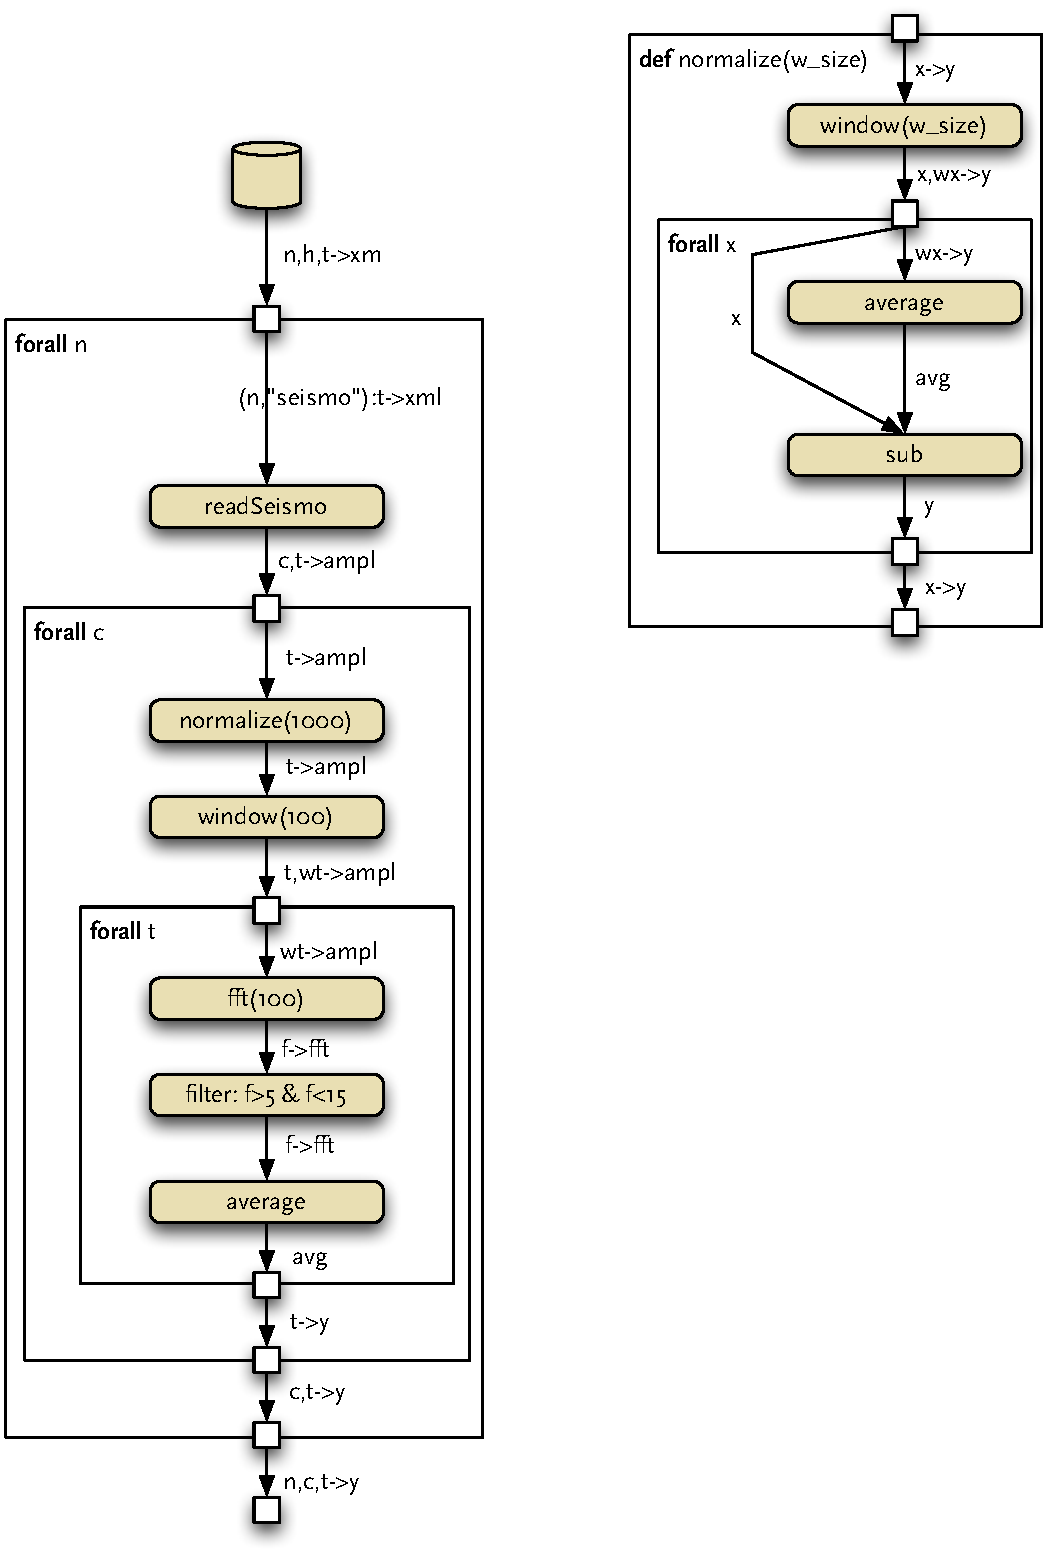
\includegraphics[width=\linewidth]{figures/seismo_bus_composition}
    \caption{Seismo analysis composition.}%
    \label{fig:seismo_bus_composition}
  }%
  \qquad
  \begin{minipage}{0.45\linewidth}%
    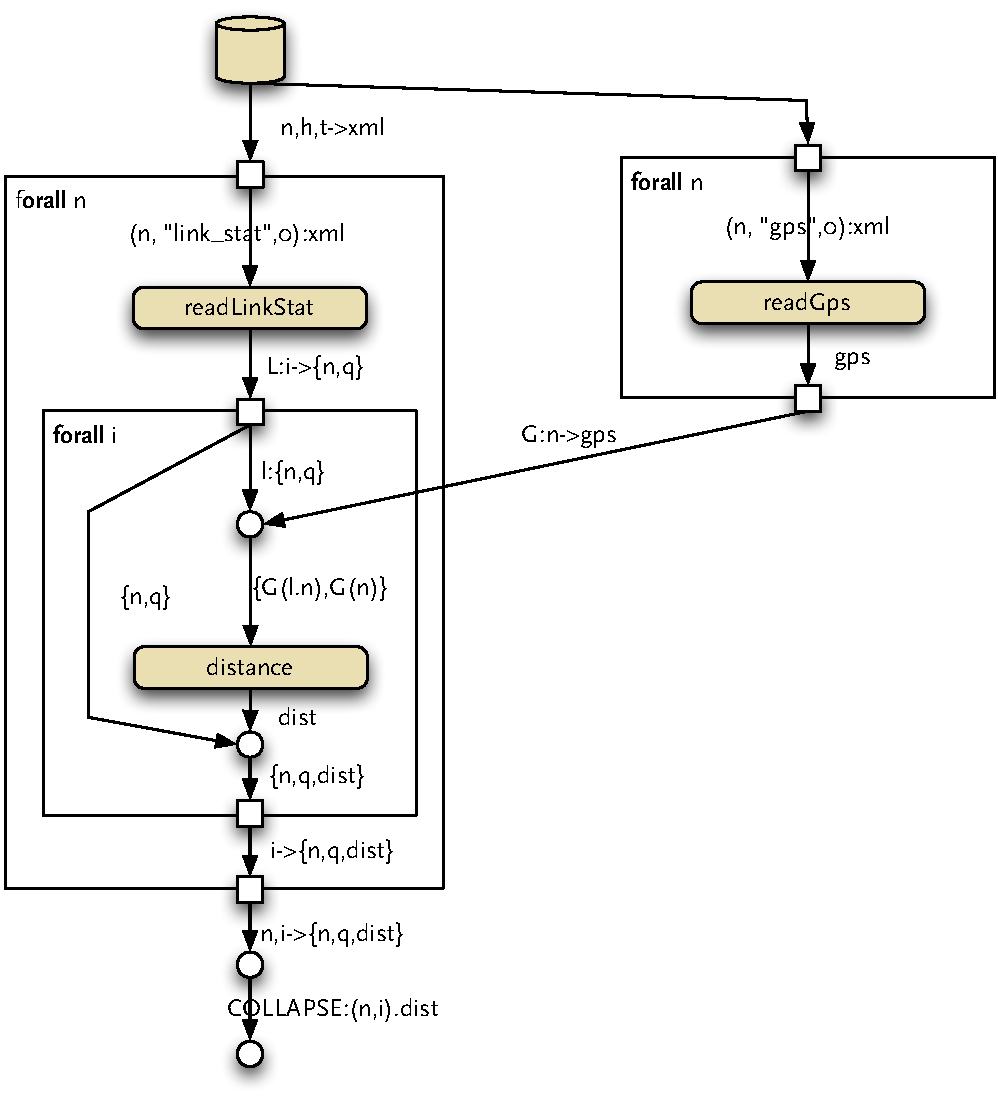
\includegraphics[width=\linewidth]{figures/link_distances_composition}
    \caption{Link distances composition}%
    \label{fig:link_distances_composition}%
  \end{minipage}
\end{figure}

Examples taken from experiments with wireless mesh networks, the experiment pictured in Fig.~\ref{fig:example_analysis_data}. The gps coordinates of two wireless nodes are siblings with the experiment time as closest common ancestor. The gps coordinates of two wireless nodes that form a link are siblings to the link quality of that link with the link as closest common ancestor; further ancestors are the nodes of the link and the experiment time.

Fig.~\ref{fig:seismo_bus_composition} and Fig.~\ref{fig:link_distances_composition} examples for the analysis of BRN ClickWatch data. These activity diagrams choreograph analysis steps (activities). Both are supposed to be performed on BRN ClickWatch data. This is are information graphs (trees). In those nodes have handlers and handlers have XML values at different points in time: hence n, h, t, xml as starting information graph. XML values are part of the information graph.

\subsection{Applications}

The described concepts of APD, information and analysis are not new and performed in many fields. What is somewhat new is the notion of traces. In complex analysis scenarios traces allow to find siblings and common ancestors that allow to put the results and intermediate results of one or multiple analysis in relation. 

In experiment scenarios, where heterogenous data is produced and analyzed, different types of data is analyzed in different analysis steps, threads of analysis steps aggregate the different types of data with each other, and with each further analysis step the created results represent information on increasingly higher levels of abstraction.

In such scenarios, it is not trivial to identify all ancestors and siblings of a resulting APD. Heterogenous data analysis produces different results. During interpretation of these results, the APDs of the different results must be related to each other. 

Example wireless mesh networks (WMN) with sensors (SN). In this scenarios we have a large number of similar (or identical) data sources: the nodes of the network. But each node produces a large number of different APDs. Different sensors, protocol entities, etc. produce all different data. Analysis in this context means that for the different data types on each of the identical nodes different threads of analysis steps are applied. The results are complex information graphs that cover different aspects of the network. Trace based knowledge about ancestors and siblings becomes key. 

A few examples from WMNs and SNs. The seismo sensors on the 100 network nodes produce time signals: one might want to compare the time signals of nodes that are geographically close to each other. Close geographic positions are common ancestors for the time signals. The nodes form links (knowledge about links is a analysis result): it is important to compare the characteristic (analysis result) of one node to the characteristic of linked nodes. Here, nodes are ancestors of the characteristics; the nodes in a link have common ancestors (the links). Looking at a the characteristics of a link or a route (connected links), it is important to identify the characteristics of all nodes in the link or the route. Looking at the time signal of one sensor, one might want to see the time signals of other sensors of that node, or nodes that have links to the node, or nodes in close proximity. Looking at a sensor reading, one might want to see node characteristics recorded at a point in time close to the time of the sensor reading. Etc. etc. etc.


